%%%%%%
%$Autor: Bauer$
%$Projekt: A25-12$
%$Dateiname: RealTimeClock.tex$
%$Beschreibung: Verwendung einer Echtzeituhr$
%%%%%%




\chapter{\ac{rtc}}\label{RTC}

\section{Einleitung}

\ac{rtc} ist eine Komponente zur Zeitmessung, die in vielfältigen Anwendungen zur präzisen Zeitangabe eingesetzt wird. Eine RTC ermöglicht es elektronischen Geräten, selbst nach einem Neustart die korrekte Uhrzeit beizubehalten. Dies wird durch eine kontinuierliche Stromversorgung erzielt, oft durch eine Batterie-Backup-Lösung \ref{fig:rtc}.

Die \ac{rtc} arbeitet unabhängig von der Hauptstromversorgung des Systems und kann mit einem geringen Stromverbrauch betrieben werden. Dank ihrer Fähigkeit, neben der Zeit auch das Datum zu verfolgen, findet sie Anwendung in vielfältigen Domänen wie Computern, Embedded Systems, IoT-Geräten und vielen weiteren. Damit sind \ac{rtc}s essentielle Komponenten für Systeme, die eine genaue Zeitmessung erfordern.
 \cite{white2011}


\section{Technische Spezifikationen}

Die folgende Tabelle \ref{tab:rtc} zeigt die wichtigsten Spezifikationen der RTC auf einen Blick. Besonders hervorzuheben ist die geringe Stromaufnahme, die ihren Einsatz in batteriebetriebenen Geräten begünstigt. Die Größe des Moduls beträgt~$140 mm\times$85~mm $~\times10mm$.

\begin{center}
	\captionof{table}{Technische Daten des  RTC-Moduls DS1307 \cite{analog2008}}
	\label{tab:rtc}
	\begin{tabular}{|l|p{8cm}|}
		\hline
		IC Chip & DS1307 \\
		\hline
		Operating Voltage & 3.3 - 5 V \\
		\hline
		Max Stromaufnahme (aktiv) & 200 µA \\
		\hline
		Max Stromaufnahme (standby) & 2 µA \\
		\hline
		Zeitgenauigkeit & ±2 ppm \\
		\hline
		Betriebstemperatur & -40 bis 85°C \\
		\hline
		Batteriebackup & CR2032 \\ 
		\hline
		Abmaße & $140 mm \times 40 mm$ $\times 10 mm$ 
	\end{tabular}
\end{center}

\begin{center}
	
\includegraphics[width=0.7\linewidth]{RTC/RTC}
	\captionof{figure}{\ac{rtc} \cite{seeedstudio2020}}
	\label{fig:rtc}
\end{center}


\begin{center}
	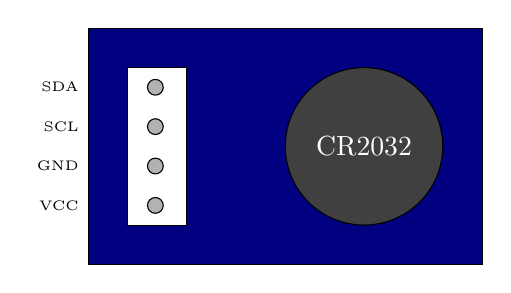
\begin{tikzpicture}
		% RTC Modul
		\draw[fill=blue!50!black] (0,0) rectangle (5,3);
		\draw[fill=white] (0.5,0.5) rectangle (1.25,2.5);
		
		\draw[fill=white!70!black](0.85,2.25) circle (0.1);
		\draw[fill=white!70!black] (0.85,1.75)  circle (0.1);
		\draw[fill=white!70!black](0.85,1.25) circle (0.1);				\draw[fill=white!70!black] (0.85,0.75) circle (0.1);
		
		
		\node[anchor=east] at (0,2.25) {\tiny SDA};
		\node[anchor=east] at (0,1.75) {\tiny SCL};
		\node[anchor=east] at (0,1.25) {\tiny GND};
		\node[anchor=east] at (0,0.75) {\tiny VCC};
		
		% Batteriehalter (runde Darstellung, auf dem Modul)
		\draw[fill=gray!50!black] (3.5,1.5) circle (1);
		\node[white] at (3.5,1.5) { CR2032};
		

		
	\end{tikzpicture}
	\captionof{figure}{RTC-Modul DS1307 nach \cite{seeed2025grove_rtc} }
		\label{rtctixz}
\end{center}

\section{Anwendungen der RTC in verschiedenen Bereichen}

\ac{rtc}s werden in einer Vielzahl von Anwendungen eingesetzt, darunter:

- \textbf{Computer}: Für die Erhaltung der Uhrzeit und des Datums.\\
- \textbf{Embedded Systems}: Als Zeitbasis für zeitabhängige Prozesse.	\\
- \textbf{IoT-Geräte}: Zur Zeitstempelung von Ereignissen für Synchronisationszwecke. \\
- \textbf{Akkubetriebene Geräte}: Minimierung des Stromverbrauchs während Standby-Phasen. \\
- \textbf{Messgeräte}: Präzise Zeitmessungen ohne ständige Verbindung zu externen Stromquellen. \\

Durch ihre vielseitige Anwendbarkeit und die Fähigkeit, kontinuierlich Zeit zu messen, ohne dass die Hauptstromquelle aktiv ist, bleiben \ac{rtc}s ein unverzichtbarer Bestandteil moderner elektronischer Systeme.

\section{Funktionsweise einer \ac{rtc}}

Eine \ac{rtc} ist eine spezielle integrierte Schaltung zur präzisen Zeitmessung, unabhängig vom Hauptsystemtakt. Sie wird typischerweise über eine Batterie (z.\,B. Knopfzelle CR1225) versorgt, sodass sie auch bei abgeschaltetem Mikrocontroller weiterläuft. \ac{rtc}s nutzen häufig einen Quarzoszillator mit 32{,}768~Hz, um die Uhrzeit durch interne Teilung auf Sekunden, Minuten und Stunden hoch zuzählen \ref{rtctixz}.

Eine \ac{rtc} kommuniziert meist über I\textsuperscript{2}C oder SPI und stellt Datum, Uhrzeit und auch Wochentag zur Verfügung. \cite{monk2017}



\section{Anwendungen von \ac{rtc} im Schlüsselkasten}

\section{Einführung}

Im Schlüsselkasten wird eine \ac{rtc} eingesetzt, um die Zeitstempel der Zugriffsereignisse zu ermöglichen. In diesem Projekt bildet die RTC zusammen mit einem RFID-System und einem Mikrocontroller das Herzstück einer intelligenten Zugriffsverwaltung. Die \ac{rtc} ermöglicht eine präzise und kontinuierliche Zeitverfolgung, auch wenn das System ausgeschaltet ist, und bietet somit eine zuverlässige Zeitbasis für das Projekt. \cite{monk2017}

\section{Funktionsweise}
Die \ac{rtc} im RFID-Schlüsselkasten speichert die genaue Uhrzeit und das Datum bei jedem Zugriff. Durch die Integration der \ac{rtc} können folgende Funktionen realisiert werden:

\begin{itemize}
  \item \textbf{Zeitstempelung von Zugriffsereignissen}: Jedem registrierten Zugriff wird ein Zeitstempel zugeordnet, wodurch nachvollziehbar bleibt, wer wann Zugang zu dem Schlüsselkasten hatte. Dies ist besonders nützlich für die Sicherheit und die Protokollierung.

  \item \textbf{Ereignisprotokollierung}: Die \ac{rtc} ermöglicht die Aufzeichnung und Verwaltung historischer Zugriffsdaten in Echtzeit. Diese Informationen können später abgerufen und analysiert werden, um Muster zu erkennen oder beispielsweise die Einhaltung von Sicherheitsrichtlinien zu überprüfen.

  \item  \textbf{Automatische Sperrzeiten}: Mit der \ac{rtc} kann programmiert werden, dass der Schlüsselkasten nur zu bestimmten Zeiten zugänglich ist, zum Beispiel während der Öffnungszeiten eines Büros oder Firma. Dies erhöht die Sicherheit, indem unzulässiger Zugang außerhalb der festgelegten Zeitbereiche verhindert wird. Diese Funktion wäre eine Erweiterung des Projekts.
\cite{monk2017}
\end{itemize}


\section{Integration ins System}

Für die Umsetzung wird die RTC zusammen mit dem RFID-Sensor direkt an den Arduino angeschlossen. Während der RFID-Sensor die Identifikation der Nutzer durch Scannen ihrer Schlüsselkarte ermöglicht, gibt die \ac{rtc} die Zeitstempel aus, die für die Verwaltung und Protokollierung der Zugriffe benötigt werden.

Das Zusammenspiel zwischen \ac{rtc} und RFID-Sensor erlaubt eine fein abgestimmte Kontrolle über den Schlüsselkasten. Durch die präzise Zeitverfolgung kann das System sicherheitsrelevante Informationen speichern.
Die Integration einer \ac{rtc} in den Schlüsselkasten macht das System zu einer leistungsfähigen und sicheren Lösung für die Verwaltung des Zugangs. Mit der Fähigkeit, ununterbrochen genaue Zeitinformationen zu liefern, sorgt die \ac{rtc} dafür, dass alle Zugriffsereignisse lückenlos dokumentiert und verwaltet werden können. \cite{adafruitRTC2020}

\section{Anbindung der \ac{rtc} DS1307 an Arduino Nano 33 BLE Sense}

	
	Die \ac{rtc} DS1307 verwendet das I\textsuperscript{2}C-Protokoll. Der Arduino Nano 33 BLE Sense besitzt separate I\textsuperscript{2}C-Pins. Die Pinbelegung \ref{RTC_PIN} ist wie folgt:
	
	\begin{center}
		\captionof{table}{Pinbelegung DS1307 am Arduino Nano 33 BLE Sense an J6 \ref{fig:TML_Cam} [eigene Darstellung]}
		\label{RTC_PIN}
		\begin{tabular}{|c|c|c|}
			\hline
				\textbf{DS1307 Pin} & \textbf{Funktion} & \textbf{Arduino Nano 33 BLE Sense Pin} \\
			\hline
				GND & Masse & GND \\
			\hline
				VCC & Versorgung & 3.3V \\
			\hline
				SCL & Clock (I2C) & SCL \\
			\hline
				SDA & Daten (I2C) & SDA \\
			\hline
		\end{tabular}
	\end{center}
	
\section{Benötigte Bibliotheken}
	
	In der Arduino IDE über den Bibliotheksverwalter sind folgende Bibliotheken zu installieren:
	
	\begin{itemize}
		\item \FILE{RTClib.h} von Adafruit
		\item \FILE{Wire.h} 
	\end{itemize}
	
\section{Einfache Anwendung}

Für den einen einfachen Code \ref{RTCSimpleCode} wird zunächst in der Funktion \PYTHON{void setup()} geprüft, ob die \ac{rtc} erreichbar ist und ob Sie ein Zeit ausgibt. In der Schleife \PYTHON{void loop()} wird dann das Datum und die aktuelle Zeit ausgegeben. Das Programm dient zur Überprüfung, ob die \ac{rtc} funktionsfähig ist.


{
  \captionof{code}{Anwendung der \ac{rtc} zur Uhrzeitabfrage}\label{RTCSimpleCode}
 \ArduinoExternal{}{../../Code/Nano33BLESense/RTC/Sample/Sample.ino}
}

\section{Uhrzeit und Datum festlegen}\label{Zeiteinstellen}

Mit dem Programm \ref{RTCSetTime} kann die aktuelle Uhrzeit und das Datum eingestellt werden.
Dazu muss vor dem hochladen die Zeile mit \PYTHON{rtc.adjust(DateTime(2000, 1, 1, 0, 6, 4));} angepasst werden. Das Format ist: Jahr, Monat, Tag, Stunde, Minute und Sekunde. 
	

{
  \captionof{code}{Programm zur Festlegung der Uhrzeit und des Datums}\label{RTCSetTime}
  \ArduinoExternal{}{../../Code/Nano33BLESense/RTC/SetTime/SetTime.ino}
}